\section{Atividades}

Neste módulo, foram realizadas atividades práticas relacionadas à
infraestrutura de certificação digital, validação de certificados SSL/TLS e
introdução ao uso de criptomoedas em ambiente controlado no Kali Linux e
Windows Server 2022.

Inicialmente foram executados procedimentos de gerenciamento de certificados
digitais em uma autoridade certificadora no Windows Server 2022, incluindo a
revogação e o cancelamento de revogação de certificados previamente emitidos.
Essas atividades permitiram compreender, na prática, o ciclo de vida de
certificados digitais e os mecanismos de controle de validade em uma
infraestrutura de chave pública (PKI).

Posteriormente, foram realizados testes de verificação de certificados Web
utilizando o protocolo \textit{OCSP (Online Certificate Status Protocol)} no
Kali Linux, permitindo analisar o estado de revogação de certificados SSL/TLS
de servidores públicos e compreender como diferentes servidores implementam
políticas distintas de resposta OCSP.

Por fim, foram desenvolvidas atividades envolvendo a criação e recuperação de
carteiras digitais de Bitcoin utilizando o software \textit{Electrum},
incluindo geração de semente criptográfica, restauração de carteira e criação
de requisição de recebimento com QR Code, demonstrando conceitos fundamentais
de segurança e custódia em criptoativos.

\newpage

\question[Atividade 9.6]{Revogação de Certificado no Windows Server 2022}

\begin{figure}[H]
  \centering
  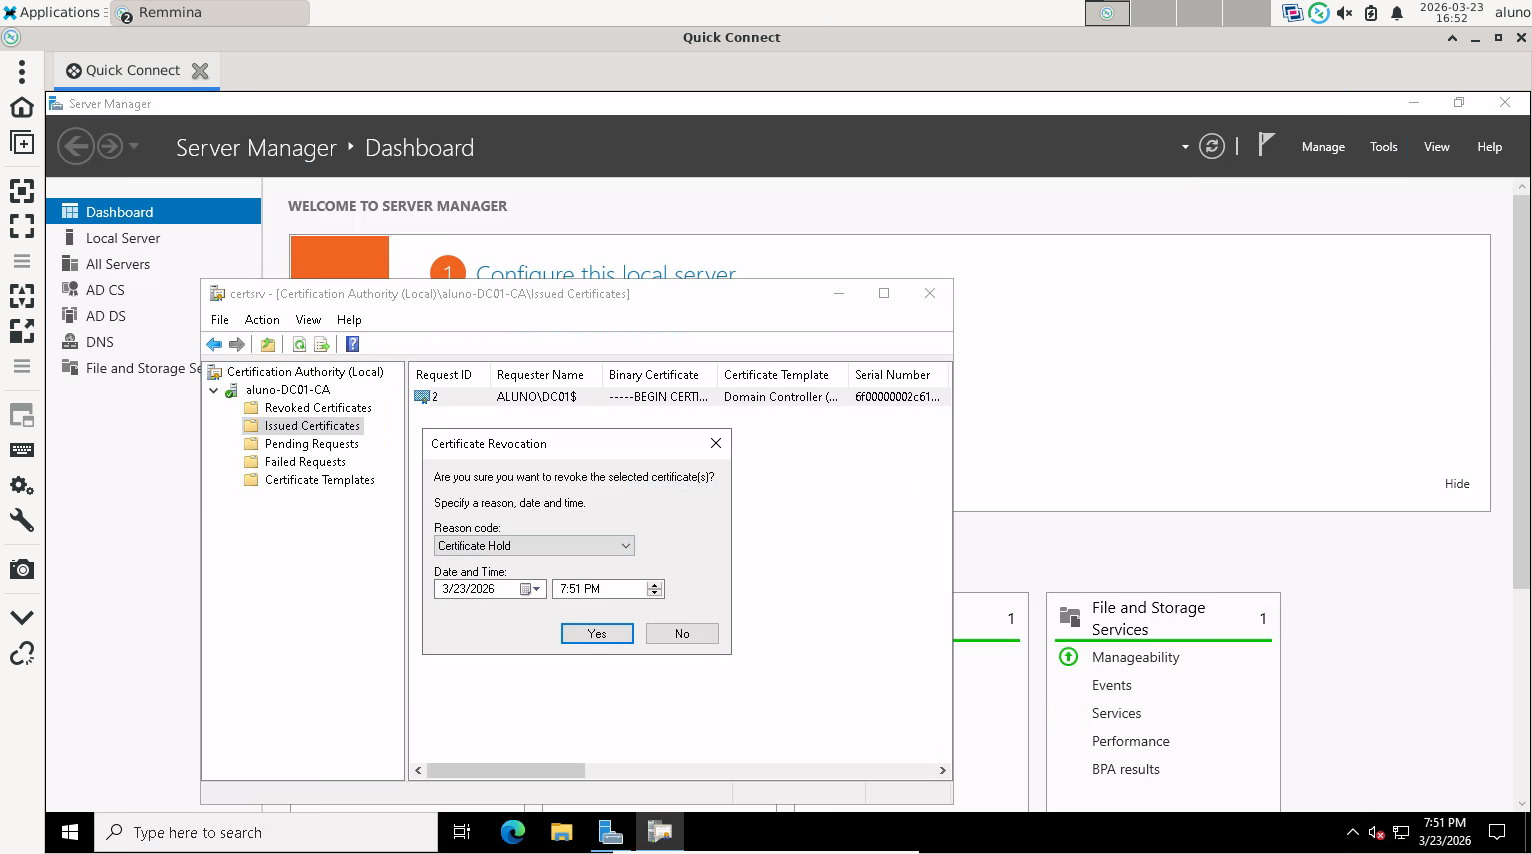
\includegraphics[width=0.99\textwidth]{./fig/fig9.6.png}
  \caption{Revogação temporária de certificado digital utilizando o motivo Certificate Hold}
  \label{fig:fig9.6}
\end{figure}

\newpage

\question[Atividade 9.7]{Cancelamento de Revogação de Certificado}

\begin{figure}[H]
  \centering
  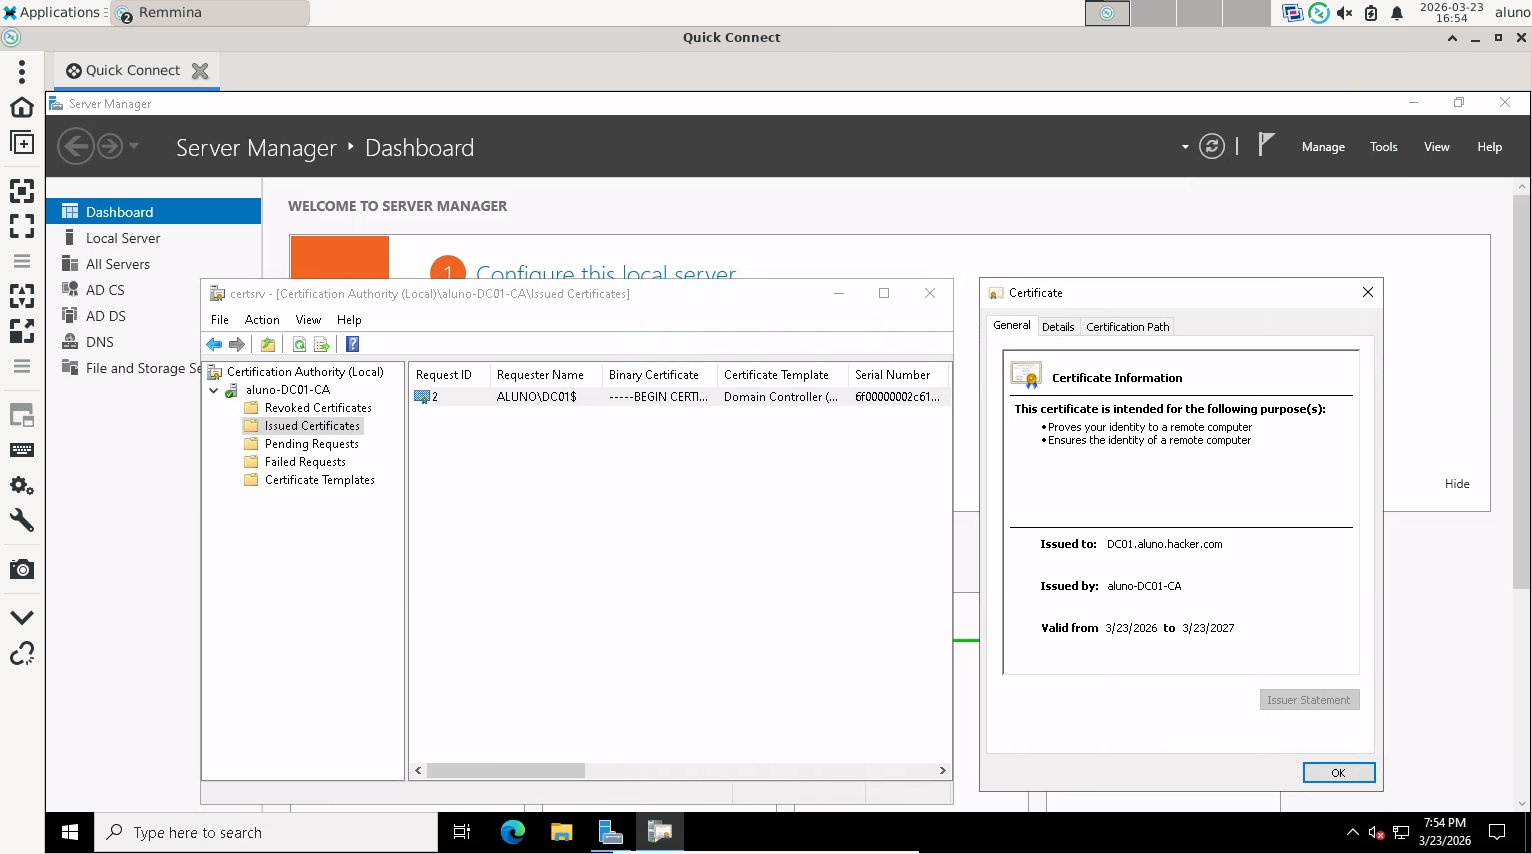
\includegraphics[width=0.99\textwidth]{./fig/fig9.7.png}
  \caption{Certificado restaurado para a pasta Issued Certificates após cancelamento da revogação}
  \label{fig:fig9.7}
\end{figure}

\newpage

\question[Atividade 9.8]{Verificação de Certificado Web com OCSP no Kali Linux}

\begin{figure}[H]
  \centering
  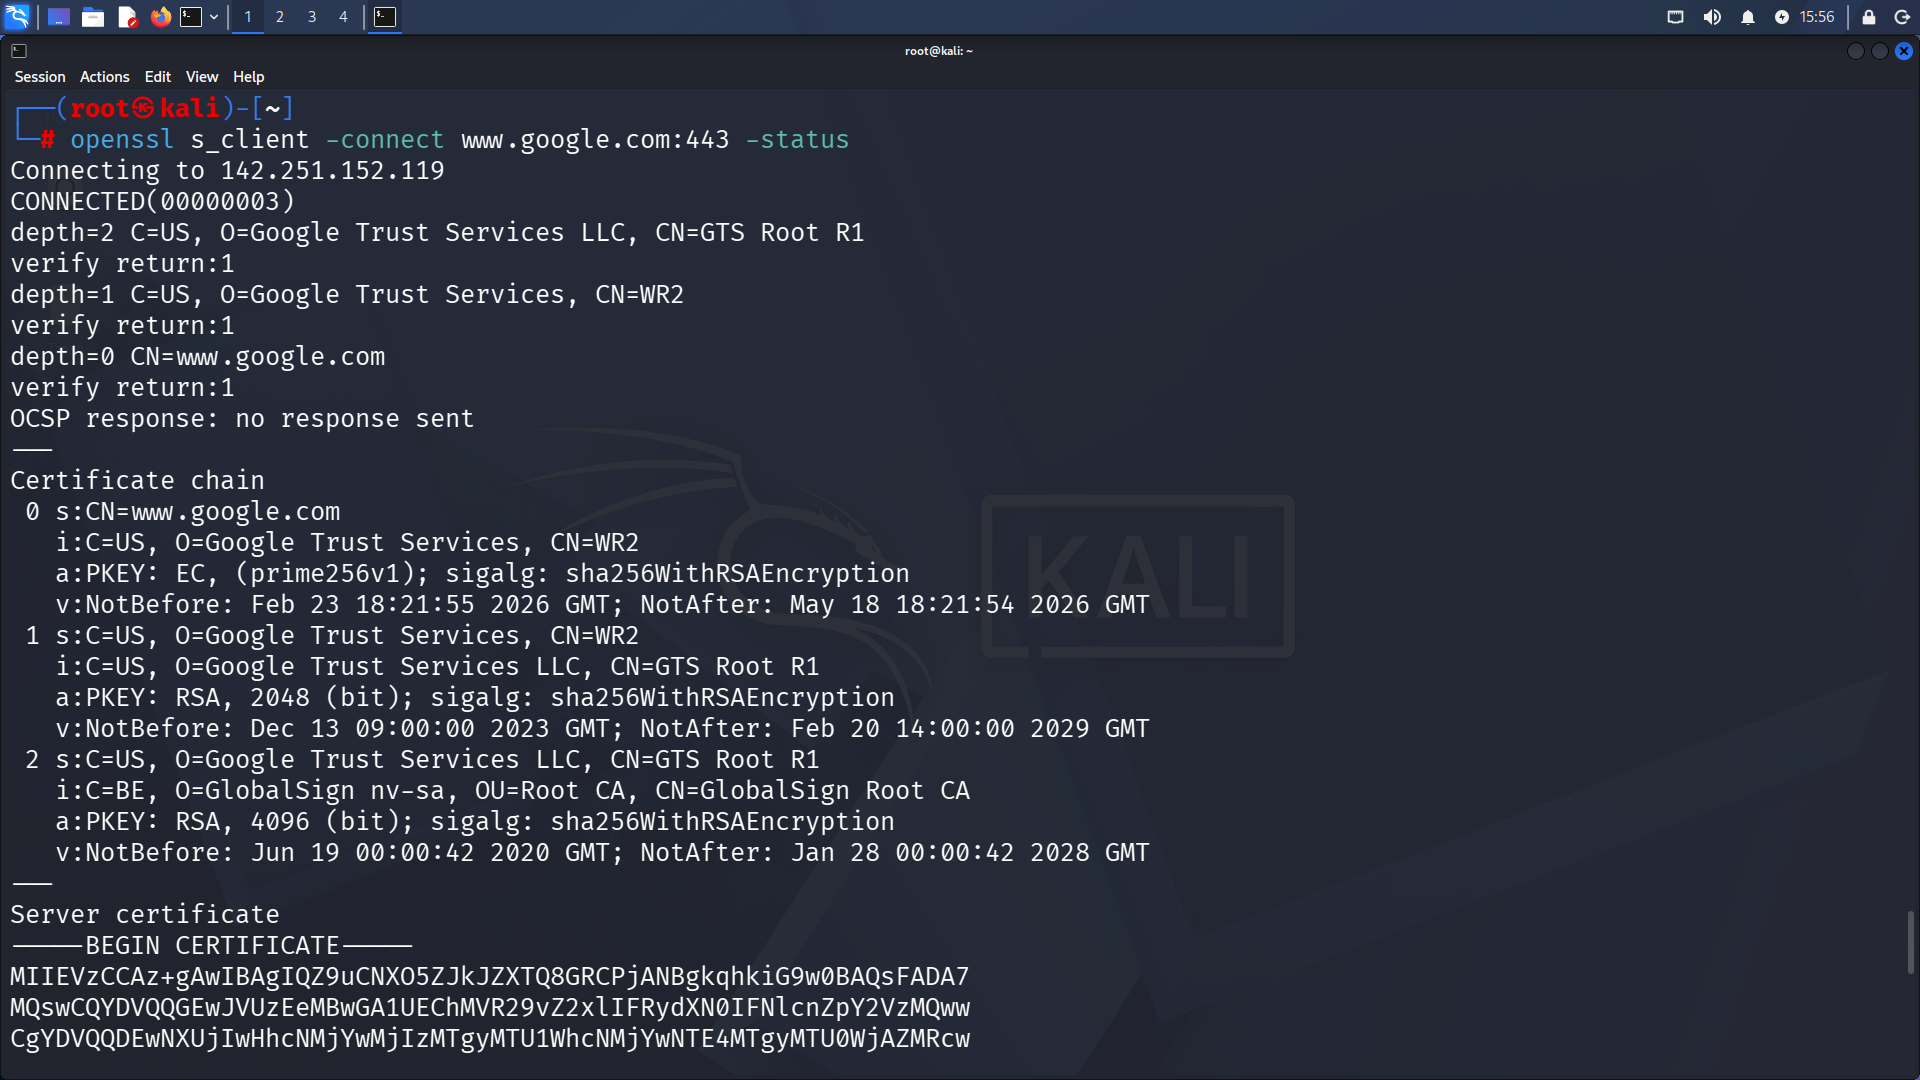
\includegraphics[width=0.99\textwidth]{./fig/fig9.8.png}
  \caption{Resultado da consulta OCSP indicando ausência de resposta do servidor}
  \label{fig:fig9.8}
\end{figure}

\newpage

\question[Atividade 9.9]{Criação de Carteira de Bitcoin com Electrum}

\begin{figure}[H]
  \centering
  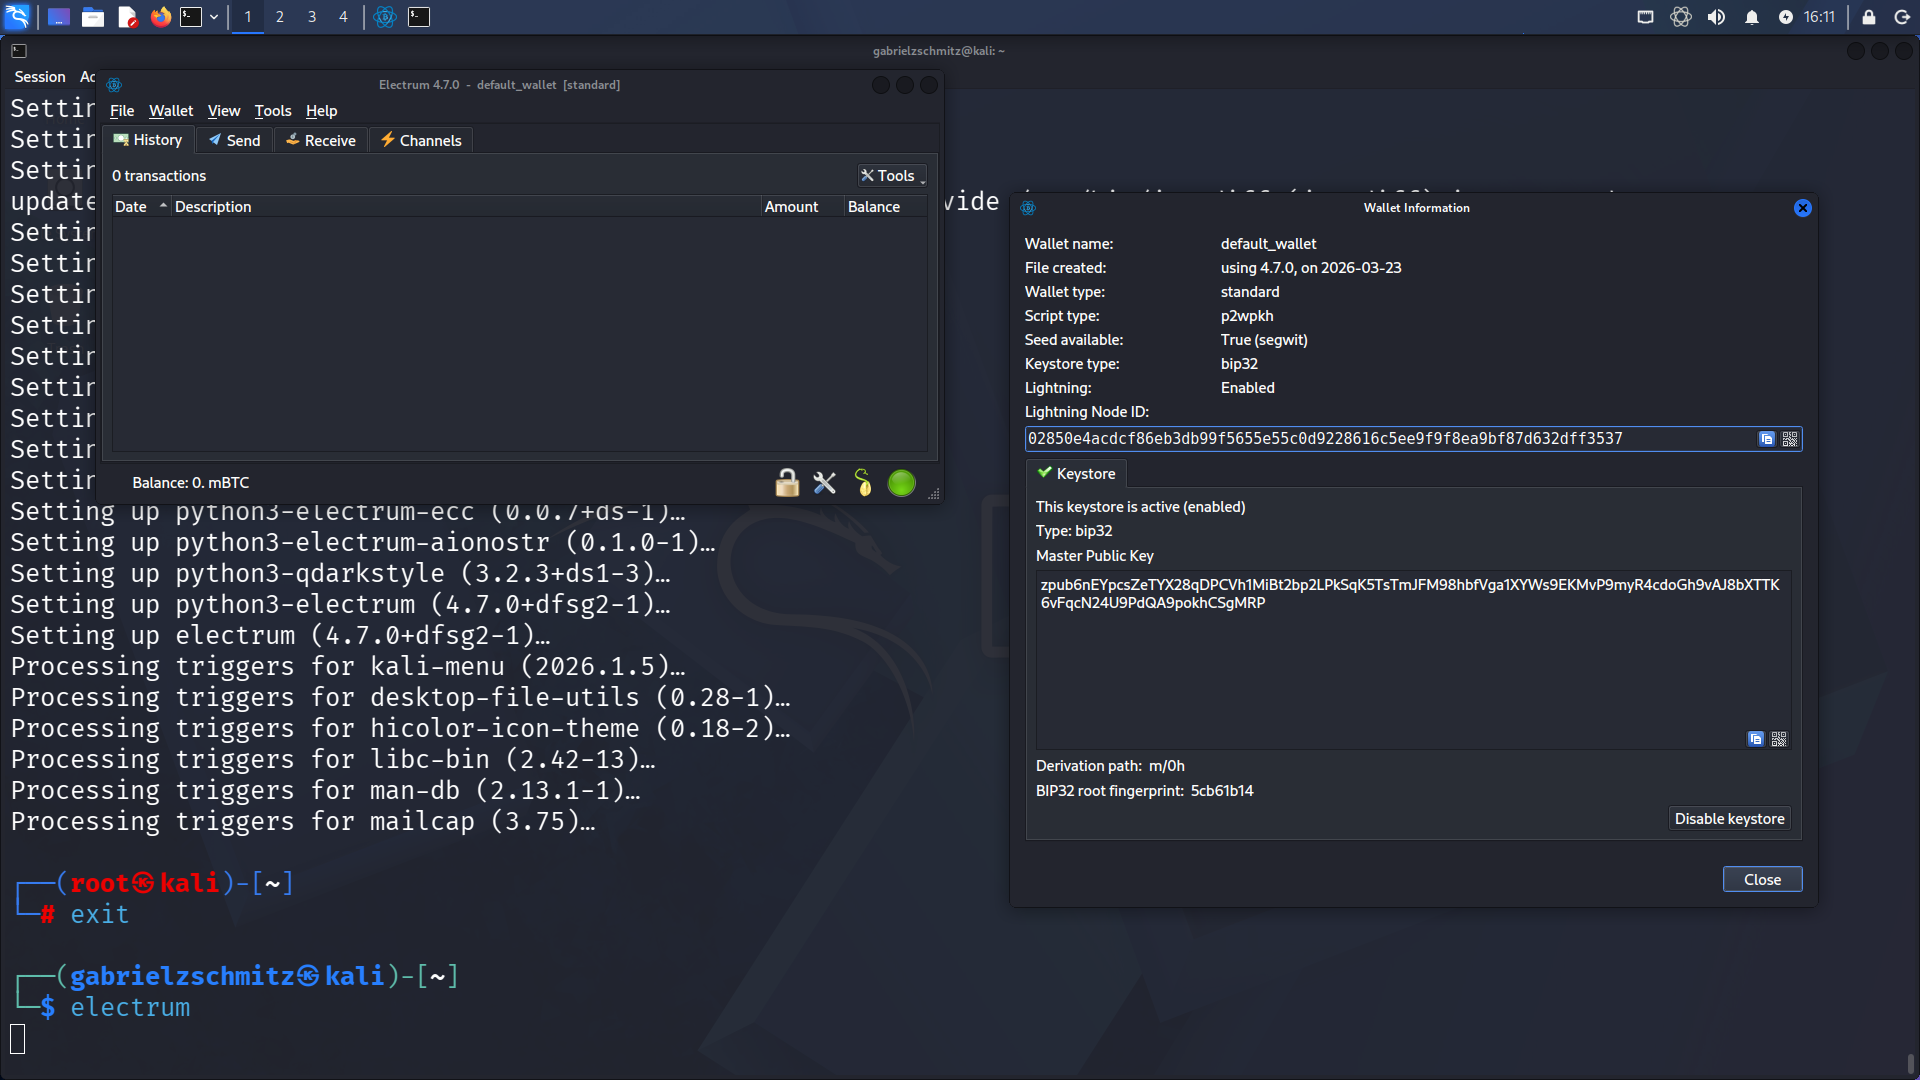
\includegraphics[width=0.99\textwidth]{./fig/fig9.9.png}
  \caption{Informações da carteira digital Bitcoin criada no Electrum}
  \label{fig:fig9.9}
\end{figure}

\newpage

\question[Atividade 9.10]{Recuperação de Carteira e Geração de QR Code para Recebimento}

\begin{figure}[H]
  \centering
  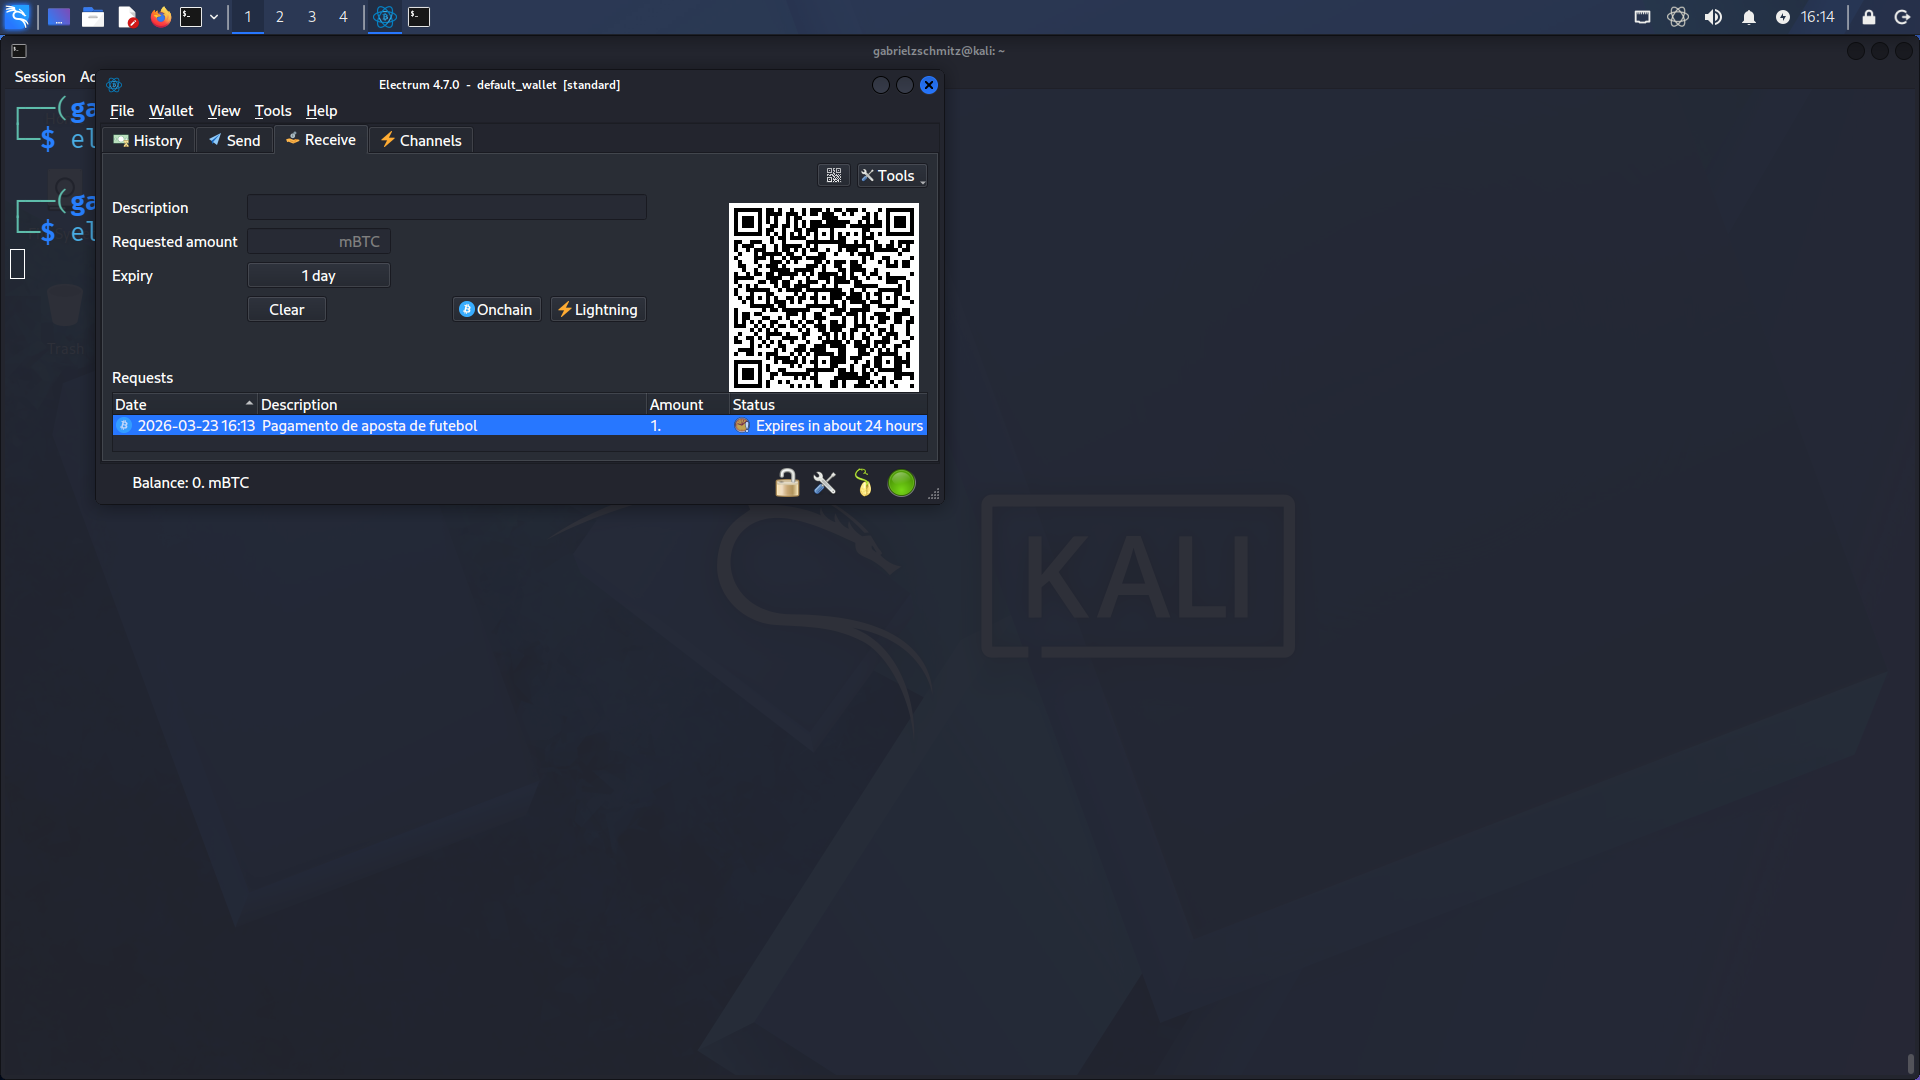
\includegraphics[width=0.99\textwidth]{./fig/fig9.10.png}
  \caption{QR Code gerado para solicitação de recebimento de Bitcoin}
  \label{fig:fig9.10}
\end{figure}
